\documentclass[12pt]{article}

\usepackage{sbc-template}
\usepackage{graphicx,url}
\usepackage[utf8]{inputenc}
\usepackage{amsmath}
\usepackage{babel}
\babelprovide[import, main]{brazilian}

\sloppy

\title{Paralelização do ACO com CUDA e OpenMP\\ para Seleção de Instâncias em Larga Escala}

\author{Raphael A. L. Soares\inst{1}, Wagner Victor A. Menezes\inst{1}, \\ Victor Gabriel R. Jácome\inst{1}, Daniel Rios Borges\inst{1} }


\address{Instituto de Informática -- Universidade Federal de Goiás
  (UFG)\\
  Caixa Postal 131 -- CEP 74001-970 -- Goiânia - GO -- Brasil
  \email{\{raphael\_alves, wagnervictor, victor\_ribeiro, daniel.rios\}@discente.ufg.br}
}

\begin{document}

\maketitle

\begin{abstract}
  Instance selection reduces dataset size while preserving classifier quality, but
  Ant Colony Optimization (ACO), although effective, has an $O(N^2)$ cost that makes it
  infeasible at large scale: the sequential C++ baseline of Magalhães et al. (2024) does
  not scale to large bases. We parallelize ACO-based instance selection in OpenMP (CPU)
  and CUDA (GPU), running the 1-NN evaluation entirely on the GPU, and assess the impact
  of thread count, scheduler and block size. On nine datasets ($\leq$5k instances) a
  24-core OpenMP run beats the GPU, but on a 253{,}680-instance base CUDA reaches
  $\sim$69$\times$ over the sequential version (vs.\ $\sim$14$\times$ for OpenMP), keeping
  the same quality ($\sim$23\% reduction, $F_1\approx0.77$). The GPU advantage is therefore
  scale-dependent: it dominates once the problem is large enough to amortize its overhead.
\end{abstract}

\begin{resumo}
  A seleção de instâncias reduz o tamanho de bases de dados preservando a qualidade de
  classificadores, mas a Otimização por Colônia de Formigas (ACO), embora eficaz, tem custo
  $O(N^2)$ que a inviabiliza em larga escala: o baseline sequencial em C++ de Magalhães et
  al.\ (2024) não escala para grandes bases. Este trabalho paraleliza o ACO de seleção de
  instâncias em OpenMP (CPU) e CUDA (GPU), com a avaliação 1-NN inteiramente na GPU, e mede o
  impacto de threads, escalonadores e tamanho de bloco. Em nove bases ($\leq$5k instâncias) o
  OpenMP em 24 núcleos supera a GPU, mas em uma base de 253.680 instâncias o CUDA atinge
  $\sim$69$\times$ sobre o sequencial (contra $\sim$14$\times$ do OpenMP), preservando a
  qualidade ($\sim$23\% de redução, $F_1\approx0{,}77$). Conclui-se que o ganho da GPU é
  dependente de escala: ela domina quando o problema é grande o suficiente para amortizar seu
  custo fixo.
\end{resumo}


\section{Introdução}

Modelos de aprendizado de máquina dependem de conjuntos de treinamento representativos, e
bases reais frequentemente contêm instâncias redundantes ou ruidosas que aumentam o custo
computacional sem agregar informação. A \textit{seleção de instâncias} ataca esse problema:
busca um subconjunto compacto dos dados que preserve (ou melhore) a acurácia de um
classificador, reduzindo tempo e recursos de treinamento~\cite{olvera2010}.

A Otimização por Colônia de Formigas (ACO)~\cite{dorigo2006} é uma metaheurística
bioinspirada eficaz para seleção de instâncias quando usada como método \textit{wrapper},
guiando a escolha de instâncias por um classificador 1-NN~\cite{cover1967}. Sua principal
limitação é o custo computacional: tanto o cálculo de distâncias quanto a avaliação 1-NN são
$O(N^2)$ no número de instâncias $N$, o que torna o algoritmo caro à medida que a base cresce.

O baseline deste trabalho, Magalhães et al.~\cite{magalhaes2024}, reescreveu o ACO de Python
para C++ e obteve ganhos expressivos de desempenho mantendo a qualidade. Entretanto, essa
versão permanece \textbf{sequencial}, e os próprios autores apontam que o alto custo
computacional ``limita sua escalabilidade, tornando-o inviável para grandes bases de dados''.
Existe, portanto, uma lacuna clara: falta uma versão \textbf{paralela} do ACO de seleção de
instâncias capaz de explorar CPUs multicore e GPUs para viabilizar o algoritmo em larga escala.

A paralelização do ACO é um tema bem estabelecido~\cite{pedemonte2011}, com implementações
eficientes em CPU multicore via OpenMP~\cite{abouelfarag2015} e em GPU via
CUDA~\cite{delevacq2013} que alcançam acelerações de uma a duas ordens de grandeza. Esses
trabalhos, contudo, concentram-se em problemas de roteamento --- sobretudo o caixeiro-viajante
--- nos quais o gargalo é a \textit{construção de caminhos}. Na seleção de instâncias o gargalo
é distinto: a avaliação 1-NN $O(N^2)$, uma carga \textit{memory-bound}~\cite{williams2009}. Não
encontramos na literatura uma avaliação sistemática da paralelização (OpenMP \textit{e} CUDA) do
ACO de seleção de instâncias em larga escala.

Implementamos o ACO de seleção de instâncias em OpenMP
(CPU)~\cite{dagum1998} e CUDA (GPU)~\cite{nickolls2008}, movendo a avaliação 1-NN inteiramente
para a GPU, e avaliamos o impacto do número de threads, do escalonador de laço e do tamanho de
bloco. Nas nove bases pequenas ($\leq$5k instâncias) o OpenMP em 24 núcleos supera a GPU, cujo
custo fixo não se amortiza; já na base CDC Diabetes de 253.680 instâncias o CUDA atinge
$\sim$69$\times$ de aceleração sobre o sequencial (contra $\sim$14$\times$ do OpenMP),
preservando a qualidade da solução ($\sim$23\% de redução com $F_1\approx0{,}77$). O resultado
central é que \textit{o ganho da GPU é dependente de escala}.


\section{Formulação do Problema}

Seja um conjunto $X = \{x_1, \dots, x_N\}$ com $N$ instâncias e $F$ atributos. A seleção de
instâncias procura um subconjunto $S \subseteq X$ que minimize $|S|$ mantendo a acurácia de um
classificador treinado em $S$. No ACO, cada uma de $K$ formigas constrói uma solução binária
(seleciona ou não cada instância) guiada por dois fatores: o \textit{feromônio} $\tau_i$, que
acumula a utilidade histórica de incluir a instância $i$, e a \textit{visibilidade} $\eta_i$,
derivada da distância média da instância às demais. A probabilidade de seleção é proporcional a
$\tau_i^{\alpha}\,\eta_i^{\beta}$. A qualidade de cada solução é medida por um classificador
1-NN aplicado sobre o subconjunto selecionado, e o feromônio é reforçado nas soluções de maior
$F_1$ e evaporado a cada iteração.

O custo computacional concentra-se em dois pontos $O(N^2 F)$: o pré-cálculo de distâncias e,
sobretudo, a avaliação 1-NN, na qual cada instância de teste busca seu vizinho mais próximo no
subconjunto selecionado. Para $N = 253{,}680$, isso significa da ordem de $10^{10}$ comparações
por iteração --- o gargalo que motiva a paralelização.


\section{Objetivos}

\begin{enumerate}
  \item Implementar o ACO de seleção de instâncias em três versões --- sequencial (baseline),
        OpenMP (CPU) e CUDA (GPU) --- com qualidade equivalente.
  \item Superar o baseline sequencial em desempenho, preservando a qualidade da seleção
        (medida por $F_1$ e taxa de redução).
  \item Avaliar a escalabilidade: em OpenMP, variando o número de threads e o escalonador de
        laço; em CUDA, variando o tamanho de bloco.
  \item Reportar o \textit{speedup} (absoluto e relativo) em bases de tamanhos distintos,
        incluindo uma base de larga escala (253.680 instâncias).
\end{enumerate}


\section{Metodologia}

\subsection{Algoritmo e implementações}

As três versões compartilham o mesmo ACO de seleção guiada por feromônio
($\alpha = \beta = 1$, taxa de evaporação $0{,}1$, $K = 64$ formigas). A construção de soluções
é \textit{embaraçosamente paralela}: cada formiga escreve apenas em sua fatia da colônia e lê o
vetor de probabilidades como dado somente-leitura, com gerador aleatório semeado por
$(\textit{iteração}, k)$ para garantir determinismo independente do paralelismo.

Na versão \textbf{OpenMP}, paralelizam-se a construção das formigas, o depósito de feromônio
(com \texttt{atomic} para evitar condições de corrida) e, principalmente, a avaliação 1-NN ---
o laço quente, que responde por mais de 98\% do tempo. Esse laço usa
\texttt{schedule(runtime)}, permitindo controlar o escalonador via a variável
\texttt{OMP\_SCHEDULE}. Na versão \textbf{CUDA}, a avaliação 1-NN roda inteiramente na GPU
(\texttt{knn\_1nn\_kernel}: uma thread por instância de teste), eliminando o transporte da
colônia $K\times N$ a cada iteração; para $N$ grande, o feromônio é mantido como vetor 1D e as
distâncias são calculadas \textit{on-the-fly}, evitando a matriz $N\times N$.

\subsection{Configuração experimental}

Todos os experimentos rodaram na \textbf{mesma máquina}: Intel Core i9-14900K (24 núcleos
físicos --- 8 \textit{performance} + 16 \textit{efficiency} --- e 32 threads) e GPU NVIDIA
GeForce RTX 4090 (24~GB). Avaliamos nove bases do baseline (de 299 a 4.981 instâncias) e a base
\textbf{CDC Diabetes Health Indicators}~\cite{cdcdataset} (253.680 instâncias, 21 atributos).
Para a comparação dos nove datasets, fixamos 100 iterações em todos os modos, garantindo
comparação justa de tempo. No experimento de larga escala (CDC) habilitamos \textit{early
stopping} (parada após 20 iterações sem melhora). As métricas são $F_1$, taxa de redução, tempo
de execução, vazão (GFLOPS) e \textit{speedup}. Para o CDC, o \textit{speedup} é normalizado por
iteração, usando como referência ($T_1$) uma execução de 1 thread da mesma campanha. O código e
os dados estão disponíveis publicamente\footnote{\url{https://github.com/phael-exe/aco-selection-parallel}}.

\subsection{Métricas}

A qualidade da seleção é avaliada por um classificador 1-NN treinado sobre o subconjunto
selecionado $S$, por meio de quatro métricas: \textit{acurácia} (fração de classificações
corretas), \textit{precisão} (fração de positivos preditos que estão corretos), \textit{recall}
(fração de positivos reais recuperados) e $F_1$, a média harmônica de precisão e \textit{recall}
($F_1 = 2\,\frac{\text{precisão}\cdot\text{recall}}{\text{precisão}+\text{recall}}$). A
compactação é medida pela \textit{taxa de redução} $1 - |S|/N$ (maior é melhor). O desempenho é
quantificado pelo tempo de execução do ACO, pela vazão da avaliação 1-NN em GFLOPS (operações de
ponto flutuante por segundo) e pelo \textit{speedup}, a razão entre o tempo de uma referência e o
tempo da configuração avaliada.


\section{Resultados}

\subsection{Desempenho em bases de pequena e média escala}

A Tabela~\ref{tab:qualidade} reporta a qualidade da seleção nas nove bases: as três
implementações convergem para soluções equivalentes (variações de $F_1$ dentro de $\sim$2\%,
compatíveis com o ruído do algoritmo estocástico), removendo de 6\% a 22\% das instâncias.
Quanto ao tempo (Figura~\ref{fig:speedup} e Tabela~\ref{tab:baseline}), o \textit{speedup} da
CUDA cresce com $N$ --- de $0{,}7\times$ na menor base a $8{,}2\times$ na maior ---, mas em
\textbf{todas} as nove bases o OpenMP em 24 núcleos é mais rápido que a GPU: o custo fixo de
lançamento de kernels e de transferência host--device não se amortiza enquanto o problema é
pequeno. Em bases de poucos milhares de instâncias, a CPU multicore é a melhor escolha.

\begin{table}[ht]
\centering
\small
\caption{Qualidade da seleção nas nove bases (classificador 1-NN, configuração sequencial; as
  três implementações convergem para qualidade equivalente).}
\label{tab:qualidade}
\begin{tabular}{lrrrrrr}
\hline
\textbf{Dataset} & \textbf{N} & \textbf{Acur.} & \textbf{Prec.} & \textbf{Recall} & \textbf{$F_1$} & \textbf{Red.\ (\%)} \\
\hline
heart\_failure & 299  & 0,926 & 0,878 & 0,896 & 0,887 & 19,4 \\
haberman       & 306  & 0,935 & 0,851 & 0,914 & 0,881 & 19,9 \\
cirrhosis      & 418  & 0,880 & 0,893 & 0,849 & 0,867 & 21,5 \\
diabetes       & 768  & 0,935 & 0,916 & 0,896 & 0,906 & 19,5 \\
tic-tac-toe    & 958  & 0,985 & 0,991 & 0,967 & 0,979 & 6,7  \\
yeast          & 1484 & 0,978 & 0,974 & 0,984 & 0,979 & 6,3  \\
vaccine        & 3152 & 0,980 & 0,961 & 0,955 & 0,958 & 12,7 \\
Employee       & 4653 & 0,867 & 0,798 & 0,821 & 0,809 & 22,2 \\
brain-stroke   & 4981 & 0,972 & 0,705 & 0,750 & 0,727 & 22,4 \\
\hline
\end{tabular}
\end{table}

\begin{figure}[ht]
\centering
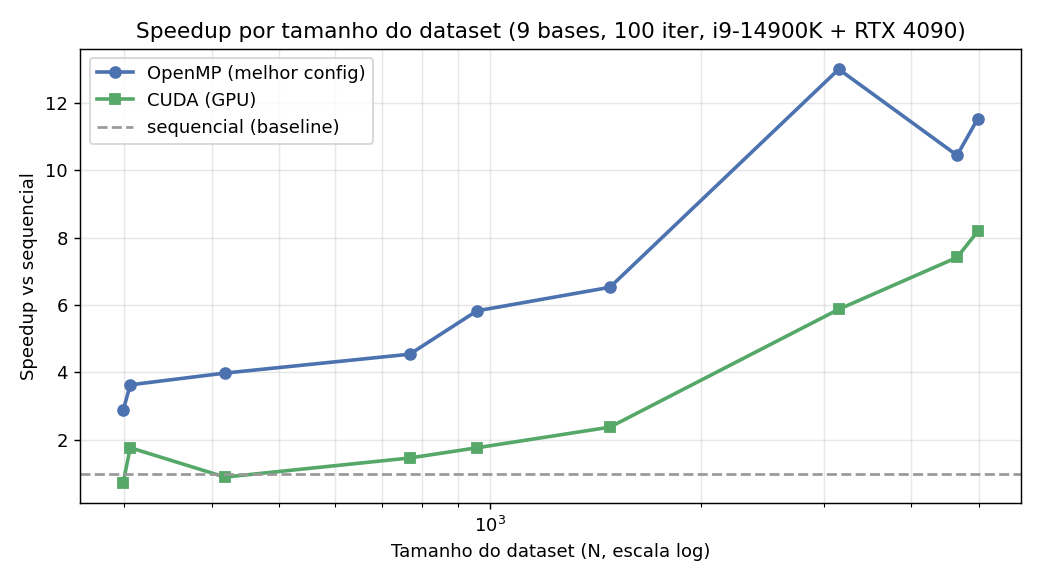
\includegraphics[width=.74\textwidth]{figs/baseline_speedup_vs_n.png}
\caption{O ganho da GPU cresce com o tamanho da base, mas até $\sim$5k instâncias o OpenMP em
  24 núcleos supera a CUDA: o custo fixo da GPU só se amortiza em escala maior.}
\label{fig:speedup}
\end{figure}

\begin{table}[ht]
\centering
\caption{\textit{Speedup} sobre o sequencial nas nove bases (100 iterações). A melhor
  configuração OpenMP é a mais rápida entre threads e escalonadores.}
\label{tab:baseline}
\begin{tabular}{lrrrr}
\hline
\textbf{Dataset} & \textbf{N} & \textbf{Seq.\ (ms)} & \textbf{CUDA} & \textbf{OpenMP (melhor)} \\
\hline
heart\_failure & 299  & 82,1    & 0,7$\times$ & 2,9$\times$ \\
haberman       & 306  & 72,2    & 1,8$\times$ & 3,6$\times$ \\
cirrhosis      & 418  & 161,4   & 0,9$\times$ & 4,0$\times$ \\
diabetes       & 768  & 275,8   & 1,5$\times$ & 4,5$\times$ \\
tic-tac-toe    & 958  & 670,6   & 1,8$\times$ & 5,8$\times$ \\
yeast          & 1484 & 861,2   & 2,4$\times$ & 6,5$\times$ \\
vaccine        & 3152 & 16439,7 & 5,9$\times$ & 13,0$\times$ \\
Employee       & 4653 & 5442,5  & 7,4$\times$ & 10,4$\times$ \\
brain-stroke   & 4981 & 7773,9  & 8,2$\times$ & 11,5$\times$ \\
\hline
\end{tabular}
\end{table}

\subsection{Efeito do escalonador OpenMP}

A avaliação 1-NN é uma carga \textit{irregular} (instâncias com vizinhos próximos terminam mais
cedo), o que favorece escalonadores que rebalanceiam a carga. A Figura~\ref{fig:sched} compara,
com 16 threads, os escalonadores \texttt{static} (partição em blocos) e \texttt{dynamic}
(distribuição sob demanda) e seus tamanhos de \textit{chunk}. Nas bases maiores, o
\texttt{dynamic} é em média $\sim$25--30\% mais rápido que o \texttt{static}, enquanto o
tamanho de \textit{chunk} (1, 2 ou 3) tem efeito secundário. O balanceamento dinâmico compensa
porque cada iteração do laço quente é pesada o suficiente para diluir o custo da fila
compartilhada. O resultado está alinhado a estudos anteriores de \textit{tuning} de
escalonadores e de número de threads em ACO paralelo~\cite{abouelfarag2015}.

\begin{figure}[ht]
\centering
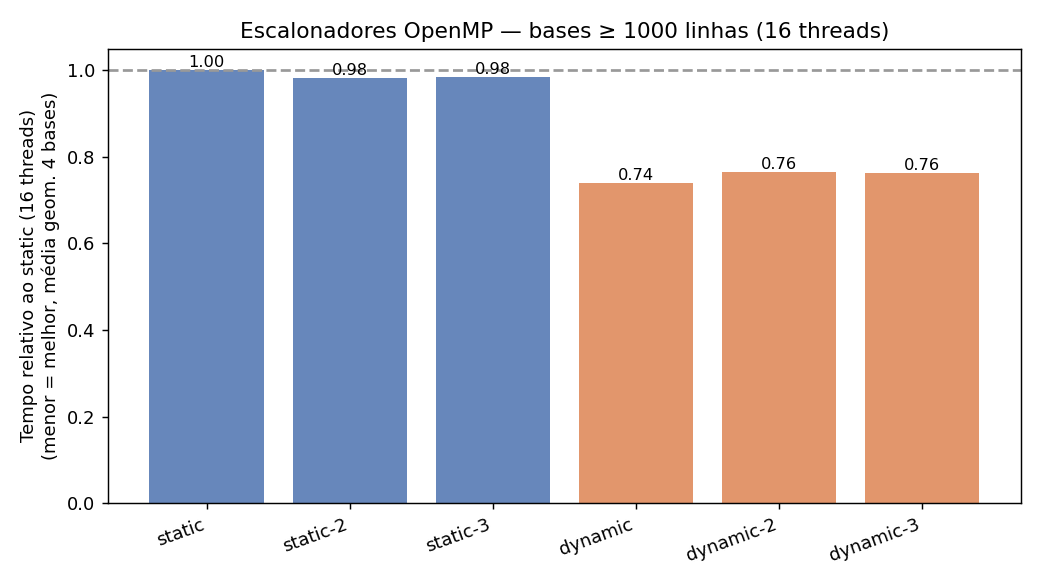
\includegraphics[width=.70\textwidth]{figs/baseline_sched.png}
\caption{Tempo relativo ao \texttt{static} (16 threads, média geométrica das bases $\geq$1000
  instâncias): o \texttt{dynamic} reduz o tempo em $\sim$25--30\%; o tamanho de \textit{chunk} é
  secundário.}
\label{fig:sched}
\end{figure}

\subsection{Desempenho na base de larga escala}

Na base CDC o quadro se inverte. O OpenMP escala bem com o número de threads
(Tabela~\ref{tab:cdcomp} e Figura~\ref{fig:cdcomp}), chegando a $\sim$14$\times$ (\texttt{static})
e $\sim$16$\times$ (\texttt{dynamic}) sobre 1 thread ao usar as 32 threads do i9-14900K; a
vantagem do \texttt{dynamic} concentra-se nos maiores graus de paralelismo. A CUDA
(Tabela~\ref{tab:cdccuda}) atinge \textbf{54--69$\times$} sobre o sequencial, executando a
campanha completa em $\sim$2~minutos --- a melhor configuração CUDA é $\sim$4,3$\times$ mais
rápida que a melhor configuração OpenMP.

\begin{table}[ht]
\centering
\caption{OpenMP na base CDC por número de threads (\textit{early stopping} em 22 iterações;
  \textit{speedup} normalizado por iteração vs.\ 1 thread; \textit{sp.}\ = \textit{speedup}).}
\label{tab:cdcomp}
\begin{tabular}{rrrrr}
\hline
\textbf{Threads} & \textbf{static (min)} & \textbf{\textit{sp.}} & \textbf{dynamic (min)} & \textbf{\textit{sp.}} \\
\hline
2  & 109,2 & 1,25$\times$  & 118,7 & 1,15$\times$ \\
4  & 60,2  & 2,26$\times$  & 57,9  & 2,35$\times$ \\
8  & 33,0  & 4,13$\times$  & 36,2  & 3,77$\times$ \\
16 & 16,5  & 8,27$\times$  & 18,1  & 7,53$\times$ \\
32 & 9,7   & 14,01$\times$ & 8,6   & \textbf{15,91$\times$} \\
\hline
\end{tabular}
\end{table}

\begin{figure}[ht]
\centering
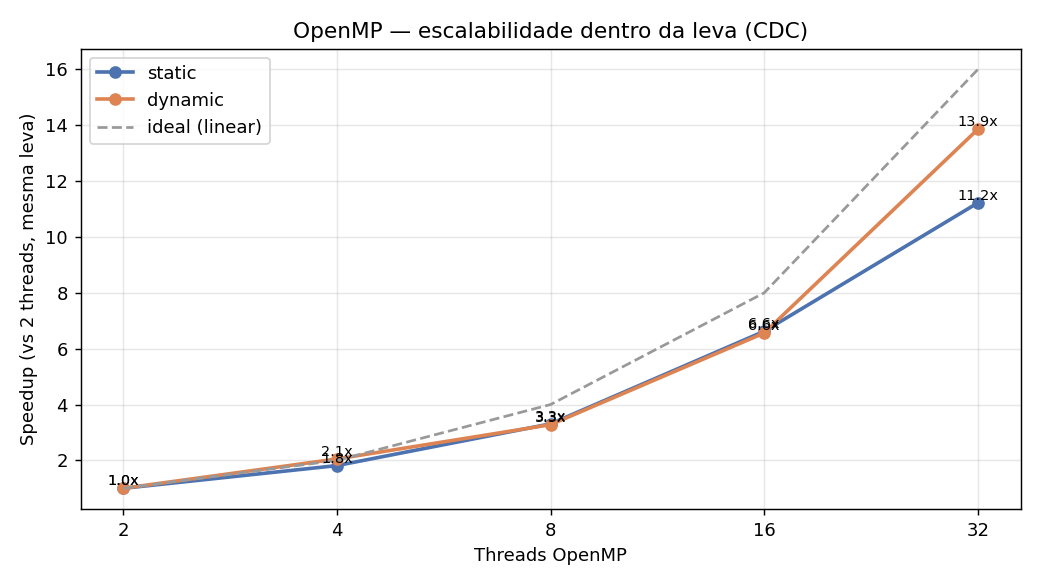
\includegraphics[width=.74\textwidth]{figs/cdc_omp_speedup.png}
\caption{Escalabilidade do OpenMP na base CDC: o \textit{speedup} relativo a 2 threads cresce de
  forma quase linear até 32 threads, com leve vantagem do \texttt{dynamic} no topo.}
\label{fig:cdcomp}
\end{figure}

A varredura de tamanho de bloco da CUDA (Figura~\ref{fig:cuda}) revela uma curva em \textbf{U}:
os extremos (bloco 32 e 1024) são mais rápidos e o meio (64--128) mais lento, com diferença de
$\sim$28\% entre o melhor e o pior. A explicação está no padrão de acesso do
\texttt{knn\_1nn\_kernel}: todas as threads leem a mesma linha de referência simultaneamente, em
\textit{broadcast}. Blocos grandes maximizam o reúso desse \textit{broadcast}, favorecidos pela
coalescência de memória~\cite{nvidiabpg}; blocos pequenos, embora de menor ocupância, mantêm o
desempenho --- pois ocupância alta não implica melhor desempenho quando há paralelismo de
instruções e de memória suficiente~\cite{volkov2010}; o meio perde nos dois efeitos. O padrão é
reprodutível (variação $<$0,2\% entre execuções repetidas), confirmando que não é ruído.

\begin{table}[ht]
\centering
\caption{CUDA na base CDC por tamanho de bloco (tempo, vazão e \textit{speedup} normalizado por
  iteração vs.\ 1 thread). A qualidade é idêntica em todos os blocos.}
\label{tab:cdccuda}
\begin{tabular}{rrrr}
\hline
\textbf{Block size} & \textbf{Tempo (s)} & \textbf{GFLOPS} & \textbf{Speedup} \\
\hline
32   & 119,7 & 573,0 & 68,4$\times$ \\
64   & 151,4 & 452,9 & 54,0$\times$ \\
128  & 149,9 & 457,3 & 54,6$\times$ \\
256  & 135,2 & 507,0 & 60,5$\times$ \\
512  & 127,9 & 536,0 & 63,9$\times$ \\
1024 & 118,5 & 578,9 & \textbf{69,1$\times$} \\
\hline
\end{tabular}
\end{table}

\begin{figure}[ht]
\centering
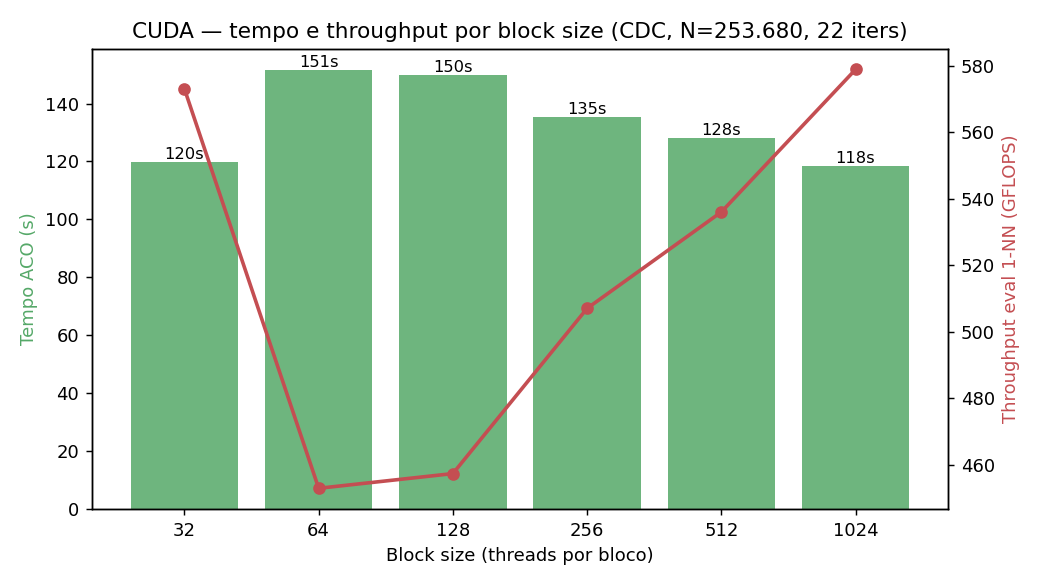
\includegraphics[width=.78\textwidth]{figs/cdc_cuda_blocksize.png}
\caption{CUDA na base CDC: a curva de tempo e vazão por tamanho de bloco tem forma de U --- os
  extremos vencem por equilibrarem reúso de \textit{broadcast} e ocupância dos SMs.}
\label{fig:cuda}
\end{figure}

Em todos os modos a solução converge para a mesma qualidade: $\sim$23\% de redução de
instâncias mantendo $F_1\approx0{,}77$ --- a paralelização altera o tempo, não o resultado. O
\textit{early stopping} reduziu cada execução para 22 iterações, economizando $\sim$78\% do
tempo sem perda de qualidade.


\section{Análise Crítica}

Os resultados sustentam a tese de escalabilidade, mas alguns pontos merecem leitura cuidadosa.

\textbf{O ponto de cruzamento depende do hardware.} A constatação de que o OpenMP supera a GPU em
bases pequenas é contingente à CPU empregada: o i9-14900K, com 24 núcleos, é particularmente
robusto. Em uma CPU mais modesta, o ponto de cruzamento se deslocaria para bases menores e a GPU
venceria antes. O resultado deve ser lido como ``a GPU compensa acima de um limiar de tamanho'',
e não como superioridade absoluta de um paradigma.

\textbf{A explicação da curva em U é fundamentada, mas não medida.} A atribuição do efeito ao
equilíbrio entre reúso de \textit{broadcast} e ocupância é coerente com a
literatura~\cite{volkov2010,nvidiabpg}, mas não foi confirmada por \textit{profiling} do nosso
kernel (ocupância alcançada, vazão de memória e taxa de acerto de cache via Nsight Compute). A
reprodutibilidade ($<$0,2\%) garante que o padrão é real, não que a causa proposta seja a única.

\textbf{O baseline de \textit{speedup} do CDC é uma escolha metodológica.} Como executar o
sequencial completo em 253 mil instâncias levaria horas, o tempo de referência ($T_1$) é uma
execução de 1 thread da mesma campanha, com o \textit{speedup} normalizado por iteração --- justo
(mesmo código e máquina), mas cuja magnitude absoluta depende dessa normalização. Valores de
\textit{speedup} entre trabalhos só são comparáveis sob a mesma metodologia.

\textbf{Heterogeneidade de núcleos.} O i9-14900K combina 8 núcleos de desempenho (com
\textit{hyperthreading}) e 16 de eficiência; a escalabilidade de 16 para 32 threads mistura esses
tipos de núcleo, tornando a curva de \textit{speedup} menos regular que a de uma CPU homogênea.

\textbf{Generalização e comparação com a literatura.} Avaliamos uma única base de larga escala, e
a taxa de redução variou de 6\% a 22\% entre os datasets --- o benefício da seleção é dependente
dos dados. Delévacq et al.~\cite{delevacq2013} reportam $\sim$23$\times$ para o ACO em GPU no
caixeiro-viajante; nosso $\sim$69$\times$ refere-se a outro problema, outra carga (avaliação 1-NN
\textit{memory-bound}) e outro hardware, não sendo diretamente comparável, mas situando-se na
faixa de uma a duas ordens de grandeza típica de implementações de ACO em GPU~\cite{pedemonte2011}.


\section{Conclusão}

Este trabalho paralelizou o ACO de seleção de instâncias em OpenMP e CUDA, preenchendo a lacuna
de escalabilidade do baseline sequencial de Magalhães et al.~\cite{magalhaes2024} e viabilizando
o algoritmo em uma base de 253.680 instâncias. O resultado central é que \textbf{o ganho da GPU é
dependente de escala}: em bases de até $\sim$5k instâncias o OpenMP em 24 núcleos é mais rápido,
enquanto em larga escala a CUDA domina, atingindo $\sim$69$\times$ sobre o sequencial e sendo
$\sim$4,3$\times$ mais rápida que a melhor configuração de CPU --- sempre preservando a qualidade
da seleção ($\sim$23\% de redução, $F_1\approx0{,}77$).

Como trabalhos futuros, destacam-se: confirmar a explicação da curva em U por \textit{profiling}
(Nsight Compute); investigar a \textit{co-execução híbrida} CPU+GPU, particionando o trabalho
entre os dispositivos; e estender a avaliação a mais bases de larga escala, aproximando o
algoritmo de aplicações reais de mineração de dados.


\bibliographystyle{sbc}
\bibliography{sbc-template}

\end{document}
